%%%%%%%%%%%% Attribution %%%%%%%%%%%%
% This template was created by 
% Chuck F. Rocca at WCSU and may be
% copied and used freely for 
% non-commercial purposes.
% 10-17-2021
%%%%%%%%%%%%%%%%%%%%%%%%%%%%%%%%%%%%%

%%%%%%% Start Document Header %%%%%%%
% In creating a new document
% copy and paste the header 
% as is.
%%%%%%%%%%%%%%%%%%%%%%%%%%%%%%%%%%%%%

\documentclass[12pt]{article}
\usepackage[utf8]{inputenc}
\usepackage[francais]{babel}
\usepackage{amsmath}


\usepackage{tikz,lipsum,lmodern}
\usepackage[most]{tcolorbox}

\usepackage{xcolor}


%%%% Header Information %%%%
    %%% Document Settings %%%%
    \usepackage[utf8]{inputenc}
    \usepackage[
        twoside,
        top=0.5in,
        bottom=0.75in,
        inner=0.5in,
        outer=0.5in
    ]{geometry}
    \pagestyle{myheadings}

%%%% Additional Commands to Load %%%%
    \usepackage{tcolorbox}
    \tcbuselibrary{skins}
    \usepackage{minted}
    \usepackage{color}
    \usepackage{tikz}
    \usetikzlibrary{calc}
    \usepackage{tabularx,colortbl}
    \usepackage{amsfonts,amsmath,amssymb}
    \usepackage{titling}
    \usepackage{mathrsfs}
    \usepackage{calc}

%%%% Commands to Define Homework Boxes %%%%
%%%% Box Definition %%%%
    \newtcolorbox{prob}[1]{
    % Set box style
        sidebyside,
        sidebyside align=top,
    % Dimensions and layout
        width=\textwidth,
        toptitle=2.5pt,
        bottomtitle=2.5pt,
        righthand width=0.20\textwidth,
    % Coloring
        colbacktitle=gray!30,
        coltitle=black,
        colback=white,
        colframe=black,
    % Title formatting
        title={
            #1 \hfill Notes:\hspace*{0.14\textwidth}
        },
        fonttitle=\large\bfseries
    }

%%%% Environment Definition %%%%
    \newenvironment{problem}[1]{
        \begin{prob}{#1}
    }
    {
        \tcblower
        \centering

        \end{prob}
    }



%%%% Document Information %%%%
    \title{Rappel (visuels) sur les vecteurs}
    \author{ \textcolor{orange}{\textbf{Sciences industrielles de l'ingénieur}}}
    \date{Janvier 2023}

%%%%%%% End Document Header %%%%%%%


%%%% Begin Document %%%%
% note that the document starts with
% \begin{document} and ends with
% \end{document}
%%%%%%%%%%%%%%%%%%%%%%%%

\begin{document}

%%%% Format Running Header %%%%%
\markboth{\theauthor}{\thetitle}

%%%% Insert the Title Information %%%
\maketitle


%%%% General Description of the Document %%%%
\begin{abstract}
L'introduction des vecteurs doit être accompagné de preuves sur leur utilité en mécanique générale. Là où, seul un \textcolor{orange}{\textbf{point}} pourrait convenir pour indiquer les connexions gratuites à la \textcolor{orange}{\textbf{wifi}} sur porte de la Vilette. Cependant, si l'on désire se rendre compte du mouvement du vent, les points ne contiennent pas assez d'information. Un point est décrit par une caractéristique : ses \textcolor{orange}{\textbf{coordonnées}}\footnote{On note \textcolor{orange}{\textbf{toujours}} les coordonnées d'un point en fonction des axes d'un repère. Exemple : $A\ =\ ( 2,4) \ ou\ A\ =\ \begin{pmatrix} 2\\4\end{pmatrix}$}, un vecteur aura trois caractéristiques, \textcolor{orange}{\textbf{sa longueur, son orientation, et son sens}} (qu'on représente avec la flèche). Il est plus instinctif d'ajouter des flèches plutôt que des points, pour indiquer le comportement du vent en Europe par exemple.
\end{abstract}

\begin{figure}[h]
    \centering
\begin{center}
     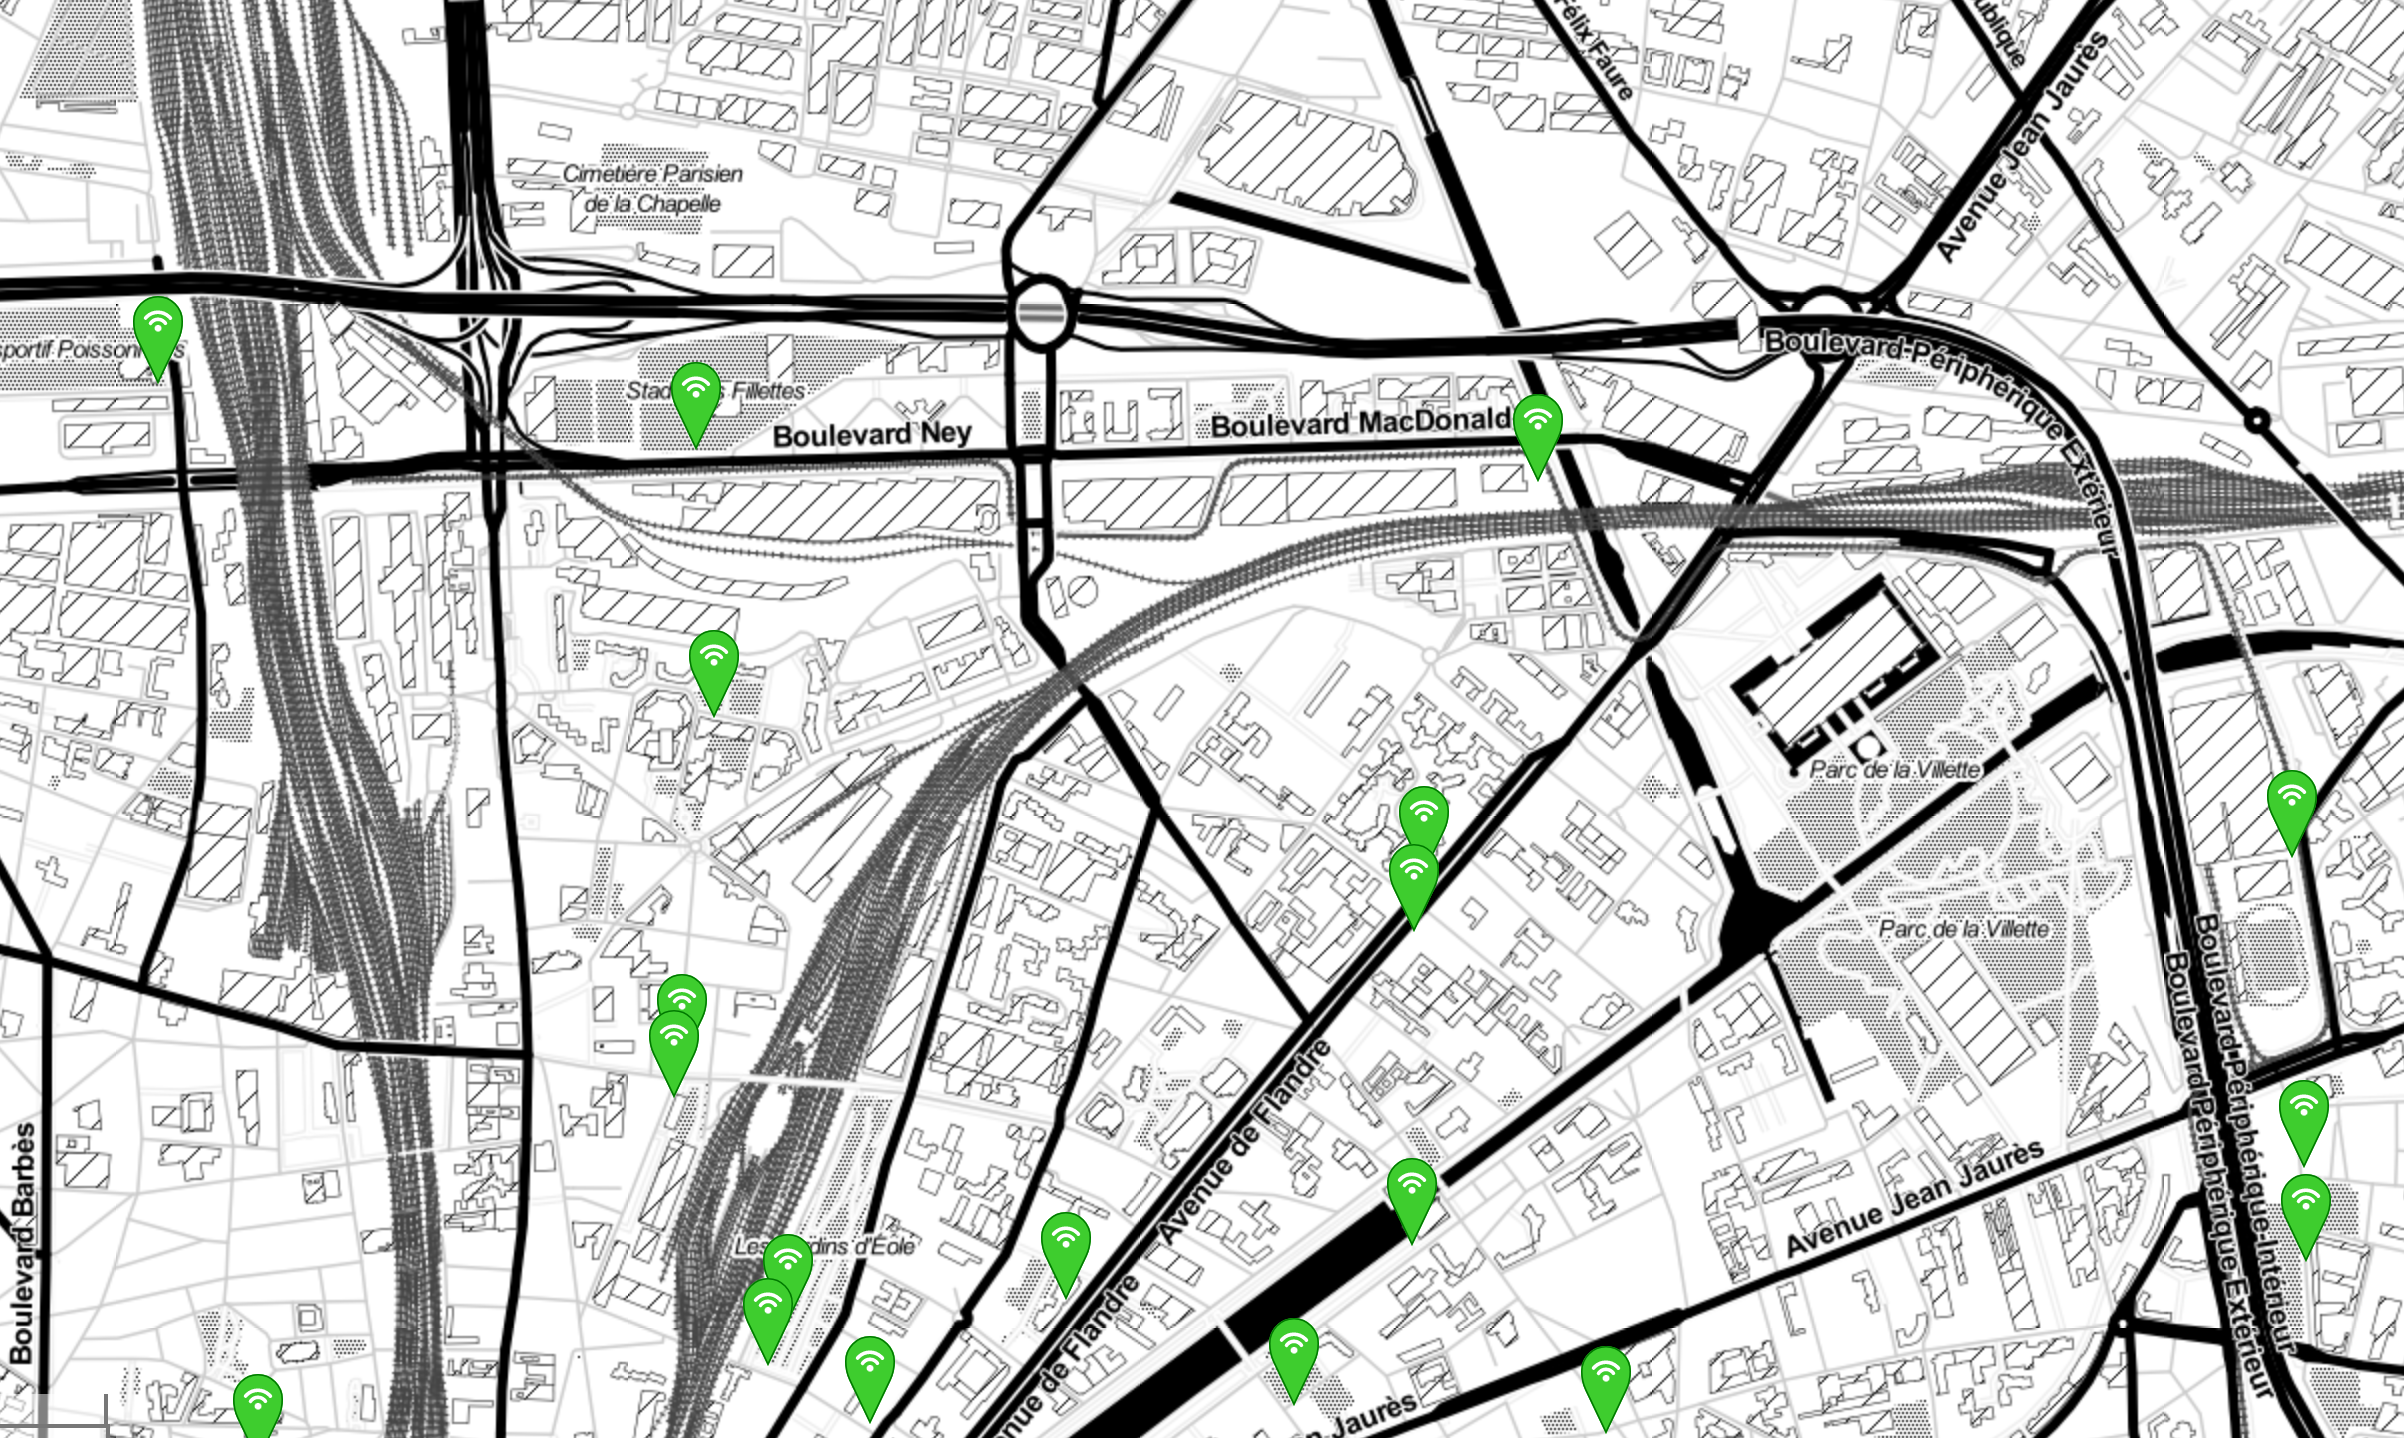
\includegraphics[width=0.45\textwidth]{Paris1.png} 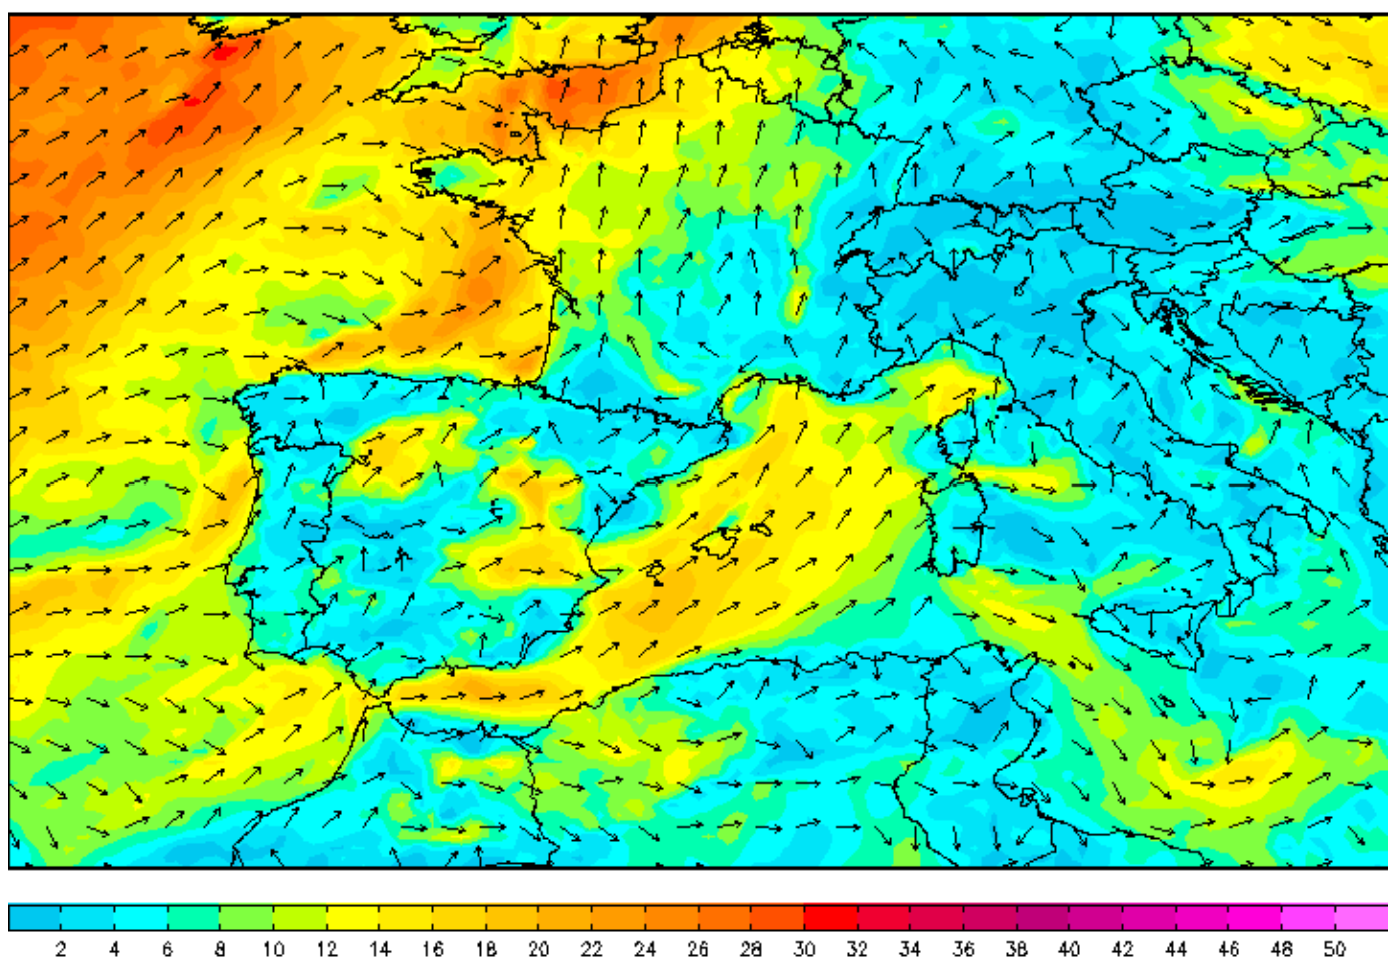
\includegraphics[width=0.45\textwidth]{Paris2.png}
     \caption{A gauche : Carte des bornes WIFI sur le quartier de la Vilette (opendata paris)}; A droite : Carte météorologique des vents (noeuds) en Europe (13:00h 07-01-2023) (freemeteo)
\end{center}
\end{figure}


%%%% Introduction to the General Template %%%%
\section{Niveau : Débutant}

\begin{problem}{\#1 Trouver les coordonnées suivantes}
    
        \begin{center}
            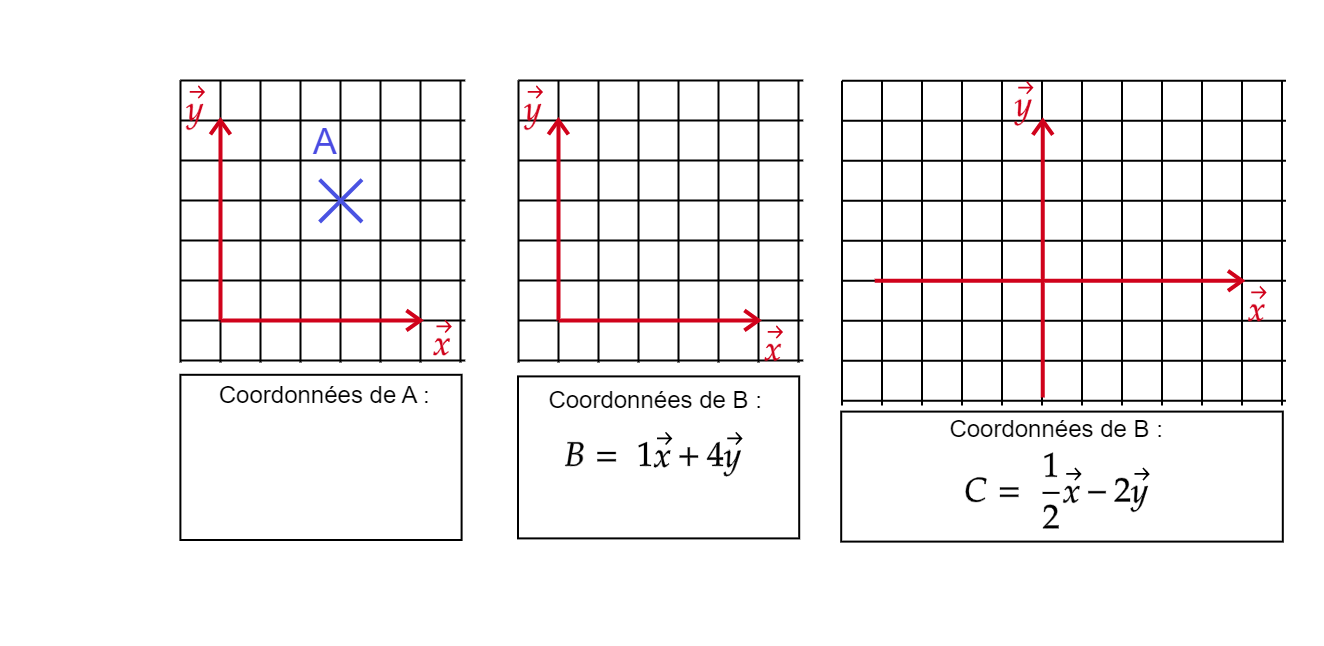
\includegraphics[width=1\textwidth]{DD1.png}
        \end{center}
    
    
Ici vous avez tracé des points, ce ne sont pas encore des vecteurs. 
\end{problem}

\noindent
Passons maintenant aux vecteurs. Le but est de connaître les différentes façon de manipuler des vecteurs, et sans se tromper ! Vous devez apprendre à les additionner, soustraire etc. Je vous conseille aussi de  \textcolor{orange}{\textbf{voir dans votre tête}} les opérations sur les vecteurs. Ce travail mental musclera votre d'abstraction mathématique et aide à la compréhension de problèmes complexe l'écrit, mais plus facile quand on les imagines.\\


\begin{tcolorbox}[colback=white!5!white,colframe=blue!75!black,title=Exemple]

\begin{minipage}{.55\linewidth}
On convient qu'il peut être plus difficile de comprendre cela :
$E=\{a,b,c\} \ ;\ A\subset E\ ,\ B\ \subset \ E\ et \\ \ E\ \cup \emptyset \ =\emptyset \ ,\ C\ =\ A\cup B\ $

Question $ C\ \subset \ E\ ?$
\end{minipage}
\begin{minipage}{.44\linewidth}
Plutôt que d'imaginer visuellement si \textcolor{orange}{\textbf{C}} est une partie de l'ensemble E : \\
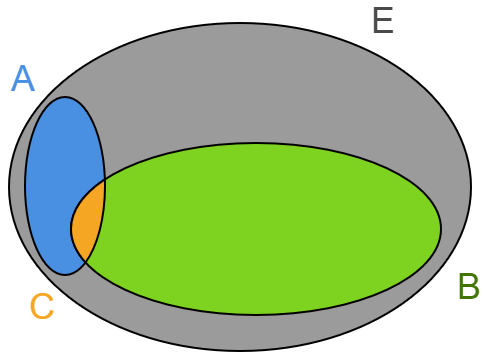
\includegraphics[width=0.4\textwidth]{DD3.png}
\end{minipage}

Réponse : Oui, \textcolor{orange}{\textbf{C}} est une partie de l'ensemble \textbf{E}, autrement dit,  
$ C\ \subset \ E\ $ est une affirmation \textbf{vraie}. Mais revenons à nos vecteurs.

\end{tcolorbox}

Retenez qu'avec les vecteurs, pour effectuer par exemple $\Vec{a}+\Vec{b}$ vous pouvez vous représenter cela visuellement.

            \begin{center}
            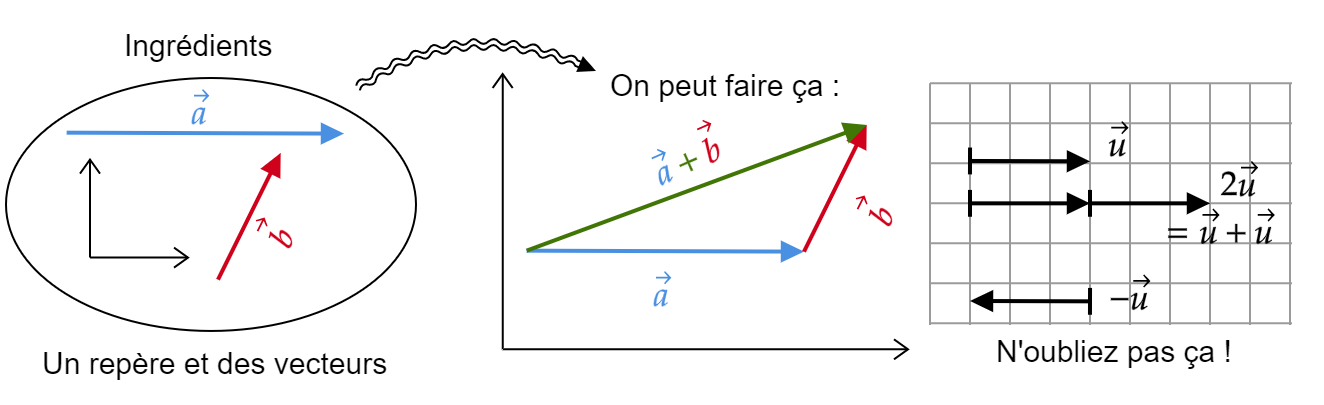
\includegraphics[width=0.9\textwidth]{DD2.png}
            \end{center}

\noindent
Ce qui est bien avec les vecteurs, c'est qu'on donne des informations selon plusieurs axes, mais on peut aussi ne considérer qu'un seul axe. 

            \begin{center}
            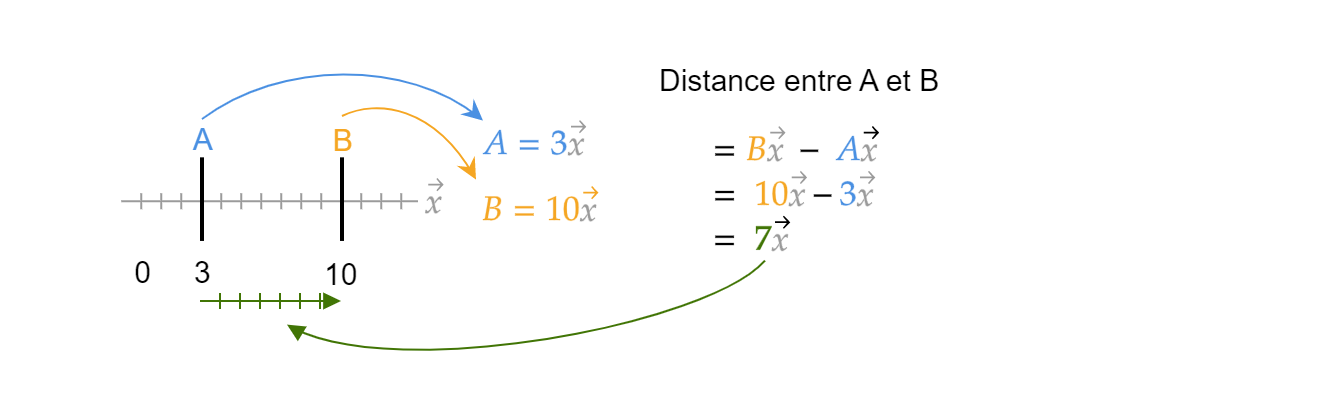
\includegraphics[width=0.9\textwidth]{DD4.png}
            \end{center}


\begin{problem}{\# 2 Calculez ou tracez la distances entres les points}
    
        \begin{center}
            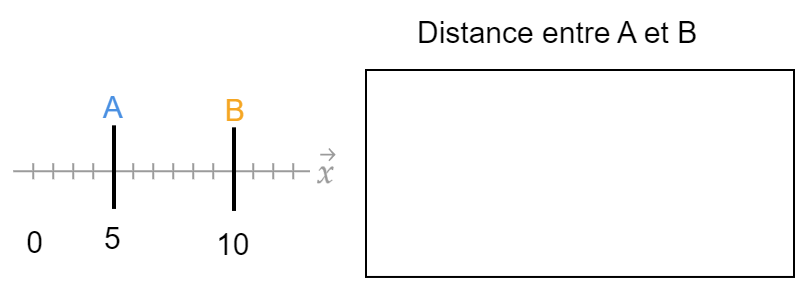
\includegraphics[width=0.7\textwidth]{DD9.png}
        \end{center}

   \begin{center}
    $C = 3 \Vec{x}$ ; $D = 9 \Vec{x}$  \hspace{2cm}          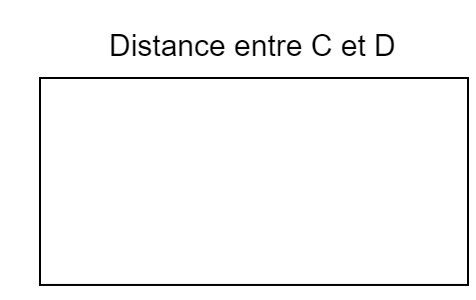
\includegraphics[width=0.4\textwidth]{DD10.png}
    \end{center}

\end{problem}


\newpage
\noindent
Vous devrez savoir ce que vous avez le droit de faire mathématiquement ou pas.

            \begin{center}
            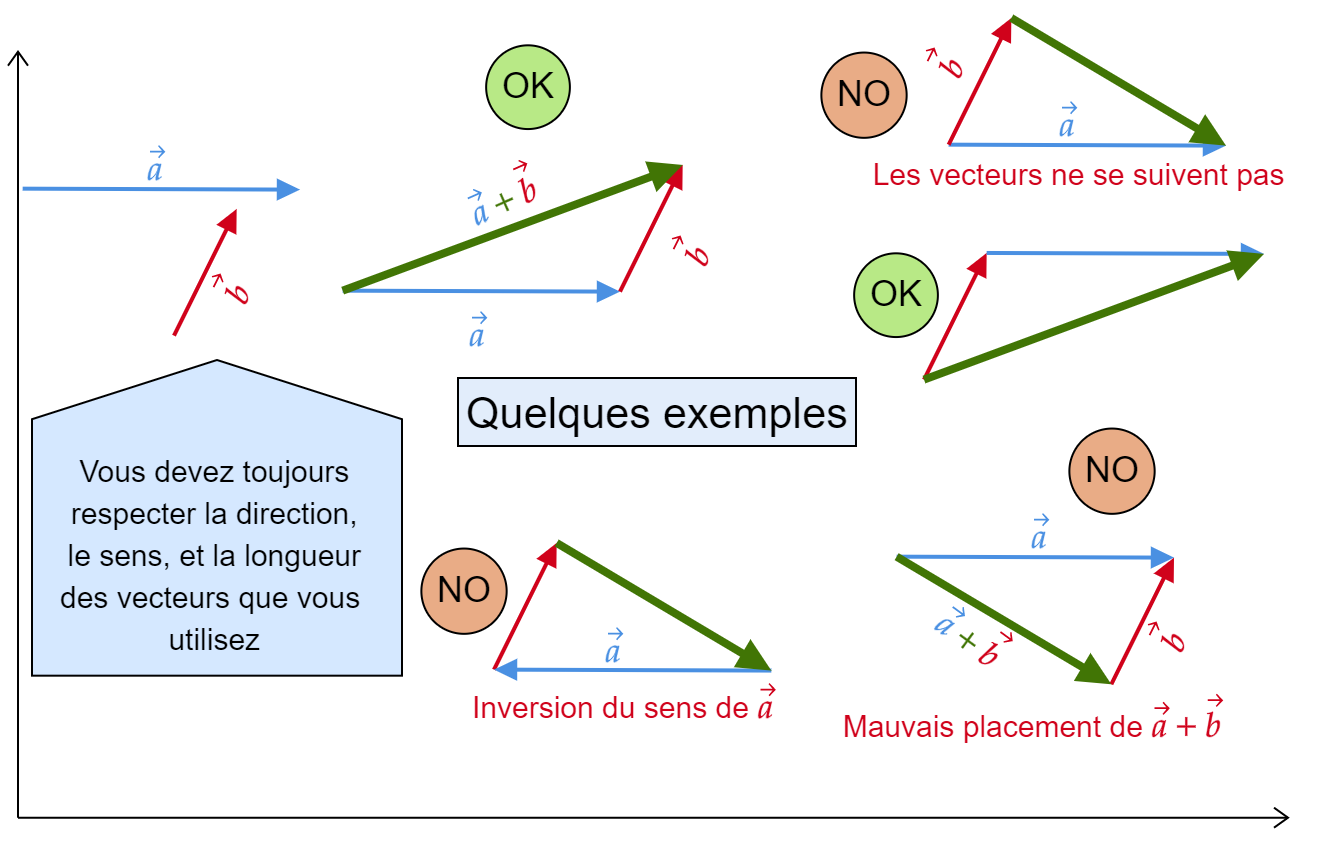
\includegraphics[width=0.9\textwidth]{DD5.png}
            \end{center}


Il y a des cas où les composantes sont égales aux vecteurs.

            \begin{center}
            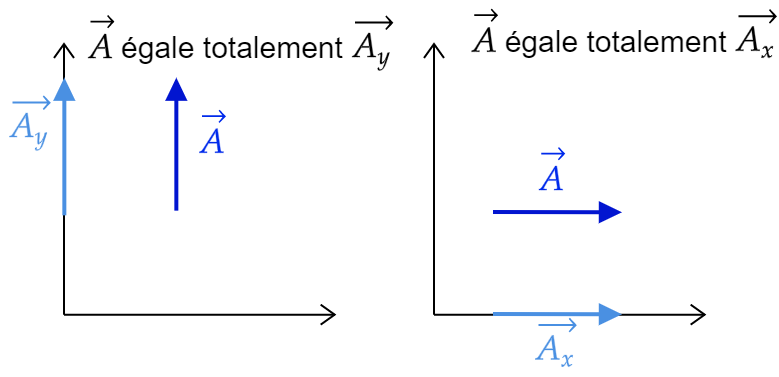
\includegraphics[width=0.5\textwidth]{DD6.png}
            \end{center}

Ce n'est généralement pas le cas :

            \begin{center}
            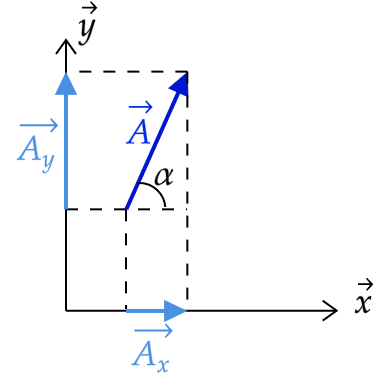
\includegraphics[width=0.3\textwidth]{DD7.png}
            \end{center}

En général, un vecteur $\Vec{A}$ dispose de différentes composantes sur les axes du repère. \\ Ces composantes peuvent être vues comme une projection de lumière, si on place une lampe parallèle à chacun des axes pour chaque vecteur.

            \begin{center}
            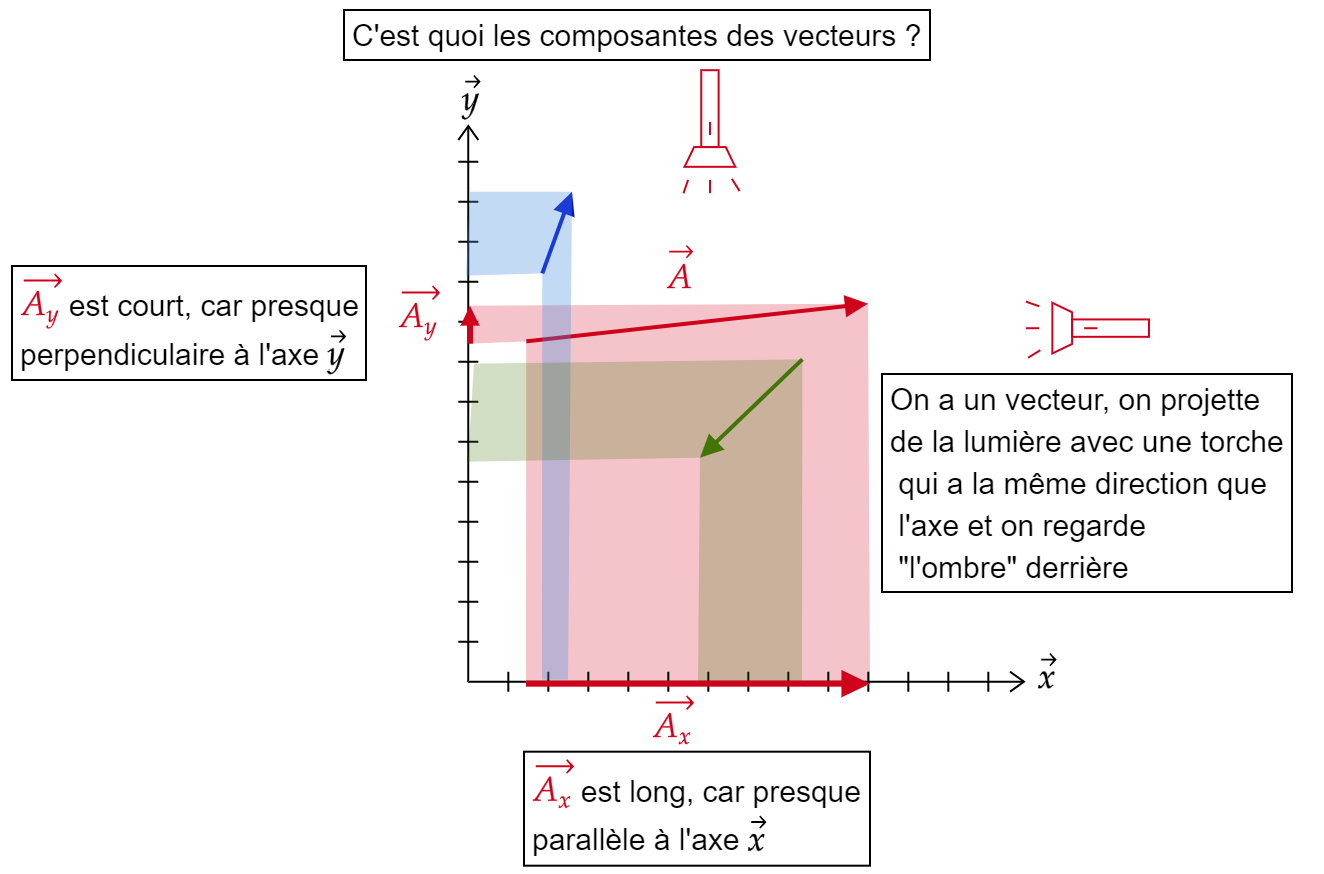
\includegraphics[width=1\textwidth]{DD81.png}
            \end{center}


\newpage

\section{Niveau : Intermédiaire}

On va s'intéresser ici aux aspect plus mathématique des vecteurs. Vous vous êtes déjà sûrement servis des formules impliquant $\cos$, $\sin$, ou des angles ($\alpha, \beta, \phi$, etc.) sur vecteurs, nous commencerons par un rappel, pour nous souvenir qu'elles viennent en général de la \textcolor{orange}{\textbf{trigonométrie}} et des formules de \textcolor{orange}{\textbf{Pythagore}} que vous connaissez déjà.

            \begin{center}
            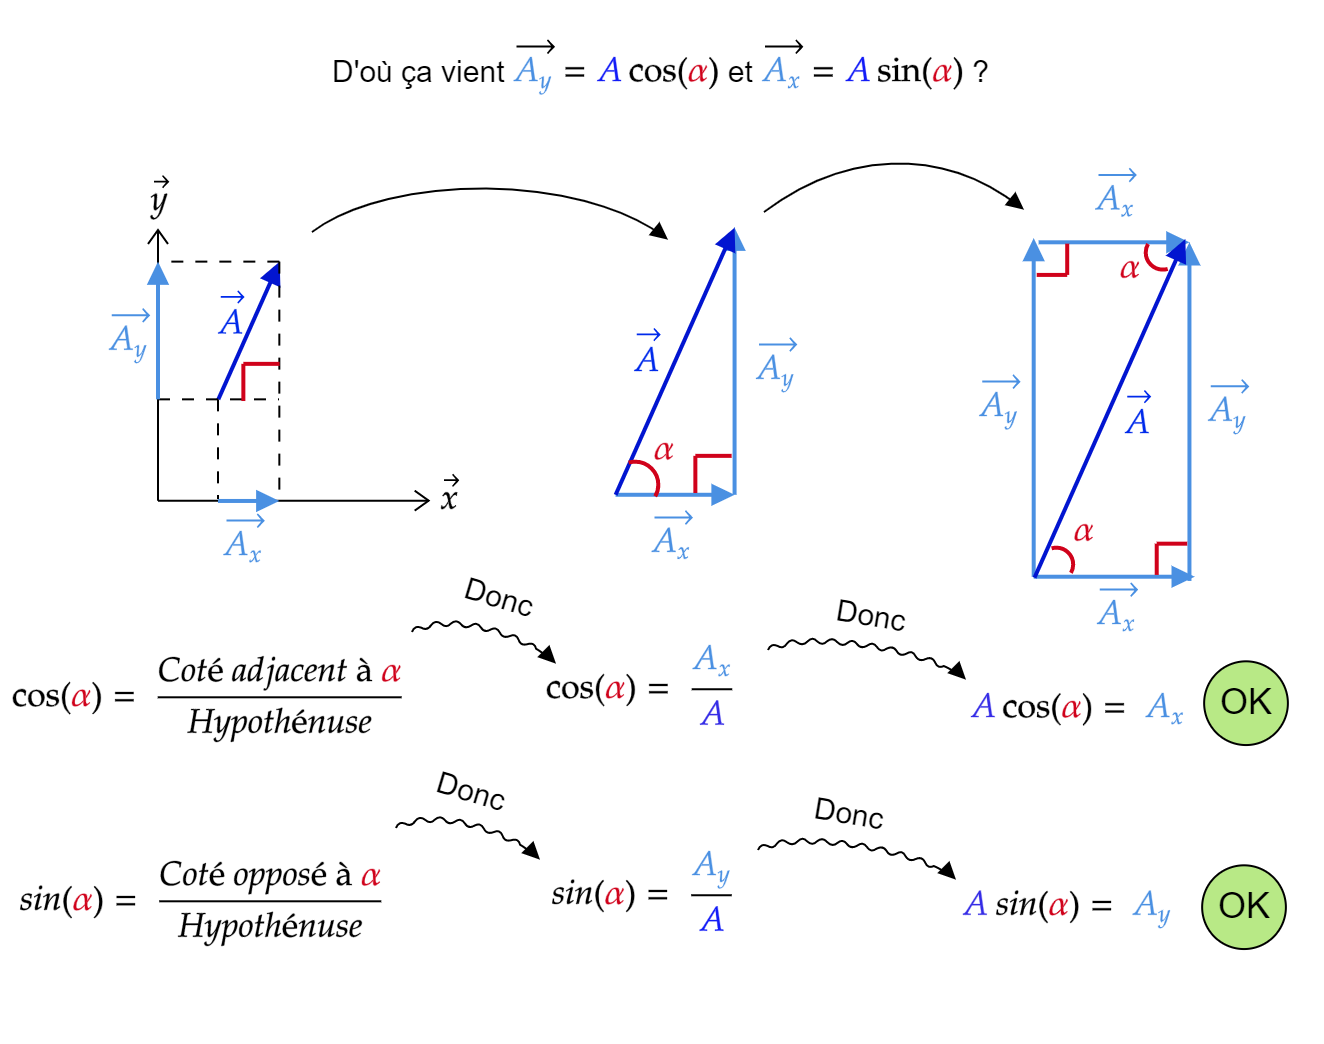
\includegraphics[width=1\textwidth]{DD8.png}
            \end{center}




Bien comprendre cela permet de savoir répondre aux nombreuses questions du type : 
\begin{minted}{latex}
Exprimer la force F en fonction de l'angle du système.
Si l'angle du système augmente, comment la force F se comporte t-elle ? 
\end{minted}

\begin{problem}{\# 2 Trouver les composantes des vecteurs}

        \begin{center}
            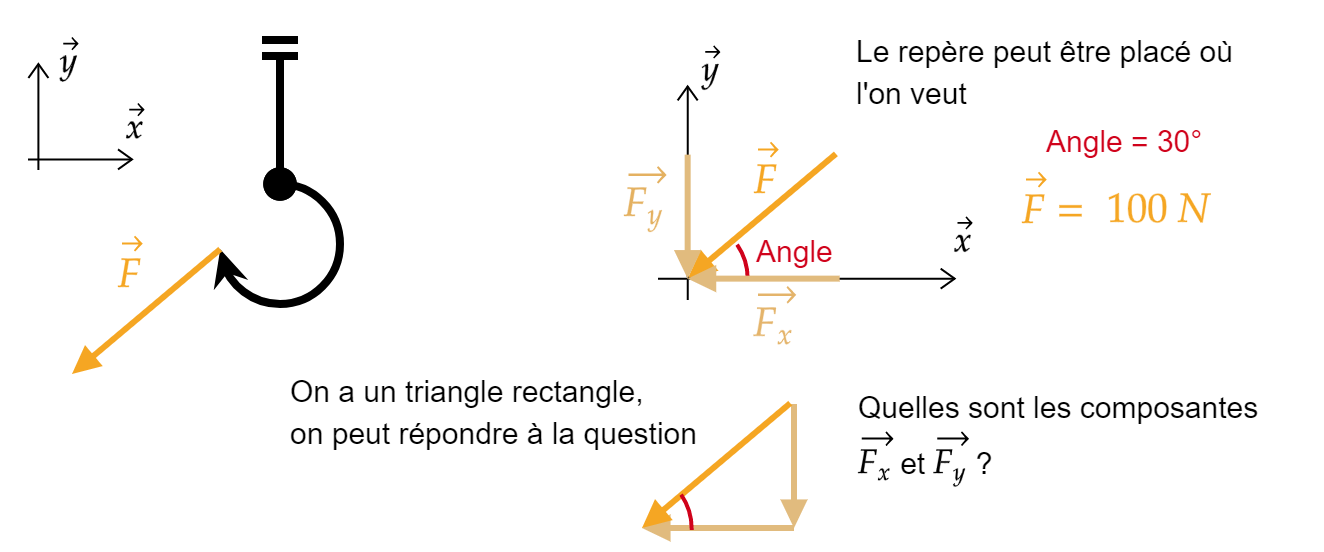
\includegraphics[width=1\textwidth]{DD11.png}
        \end{center}
    
    
Une fois qu'on a bien posé le problème, ce n'est que des math. \\

Deux personnes tirent sur une ficelle reliée à un point fixe. Calculez les composantes de $\Vec{F_1}$ et $\Vec{F_2}$ à l'aide des données.

        \begin{center}
            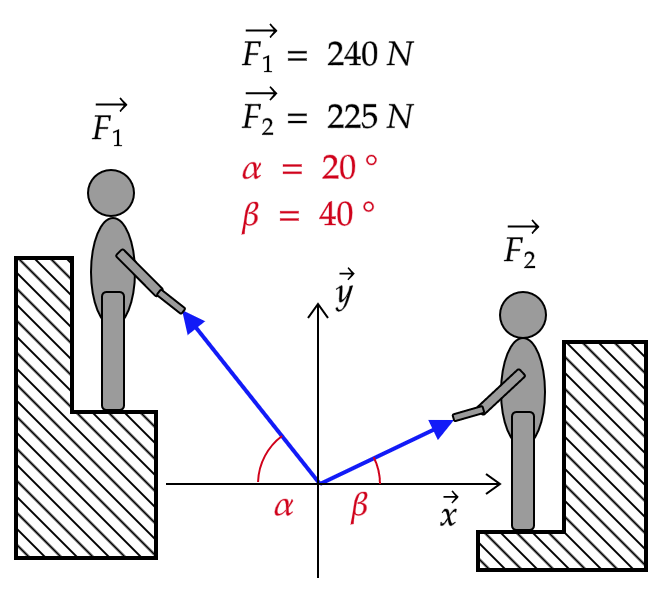
\includegraphics[width=0.6\textwidth]{DD12.png}
        \end{center}


\end{problem}



\section{Niveau BTS}




\begin{minipage}{.55\linewidth}
Un vecteur est caractérisé par :
\begin{itemize}
    \item Son point d’application A,
    \item Sa direction ($\Delta$) (ou droite support),
    \item Son sens (le signe)
    \item Sa norme A (ou intensité, ou longueur)
    \item Ses composantes.
\end{itemize}
\end{minipage}
\begin{minipage}{.44\linewidth}
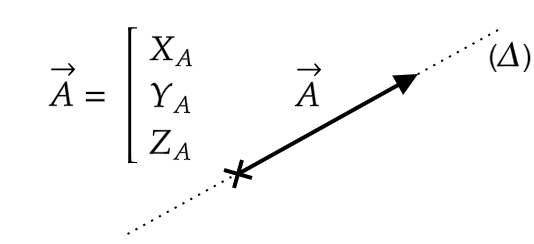
\includegraphics[width=0.8\textwidth]{DD20.png}
\end{minipage}


\begin{tcolorbox}[colback=white!5!white,colframe=blue!75!black,title=Exemple]

Vous devrez connaître le vocabulaire mathématique pour éviter les erreurs de compréhension en examen. 

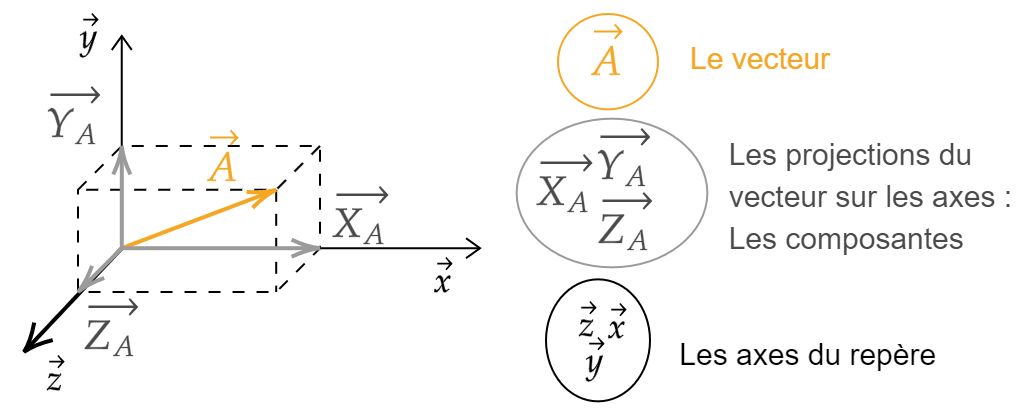
\includegraphics[width=0.8\textwidth]{DD21.png}

Notons ici que le repère est constitué de 3 axes $\Vec{x}, \Vec{y}, \Vec{z}$. Ces 3 vecteurs, seront en grande majorité tous \textcolor{orange}{\textbf{unitaires}}, c'est à dire que leur norme vaut 1 ($\Vert \vec{x}\Vert \ =\ 1$). On peut donc utiliser ces vecteurs unitaires pour exprimer un vecteur. 

\end{tcolorbox}

\subsection{Le produit scalaire}
Si on prend deux vecteurs $\Vec{u}$ et $\Vec{v}$ dans un repère plan (avec seulement 2 axes), on dira que le \textcolor{orange}{\textbf{produit scalaire}} de $\Vec{u}$ par $\Vec{v}$ (qu'on va noter $\Vec{u}.\Vec{v}$) est égal à : 
\begin{itemize}
    \item Soit 0 si l'un des deux vecteurs est nul, \\
    $\Vec{u}.\Vec{v}=0$
    \item Soit  $\Vec{u}.\Vec{v}=\Vert\vec{u}\Vert \times \Vert\vec{v}\Vert \times \cos{(\Vec{u},\Vec{v})}$ dans les autres cas.
\end{itemize}


\subsection{Le produit vectoriel}
        \begin{center}
            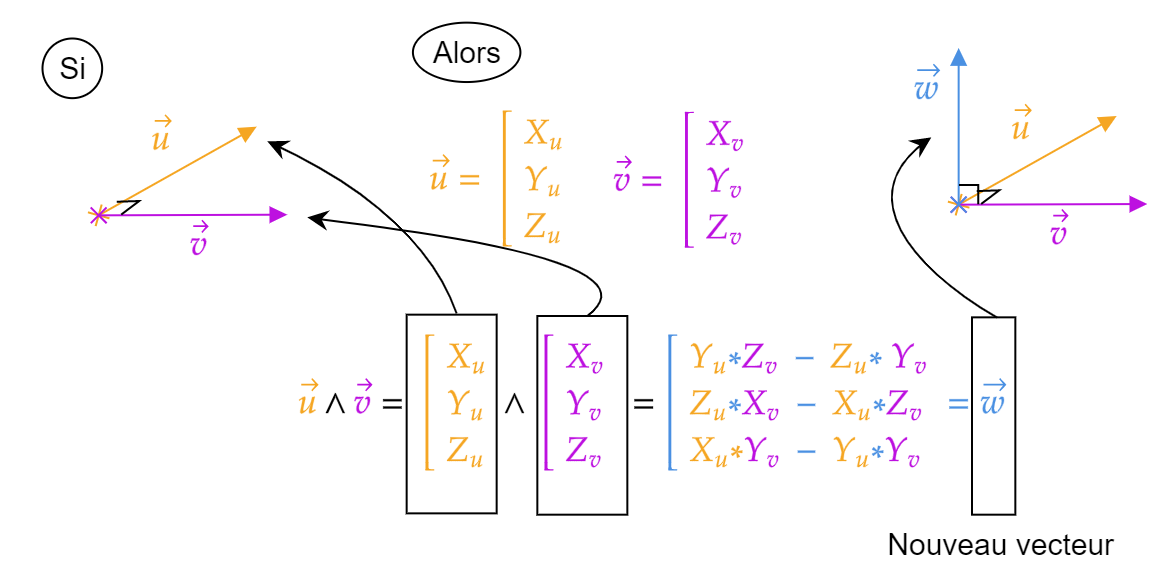
\includegraphics[width=0.8\textwidth]{DD24.png}
        \end{center}


\section{Rappel Torseurs}
        \begin{center}
            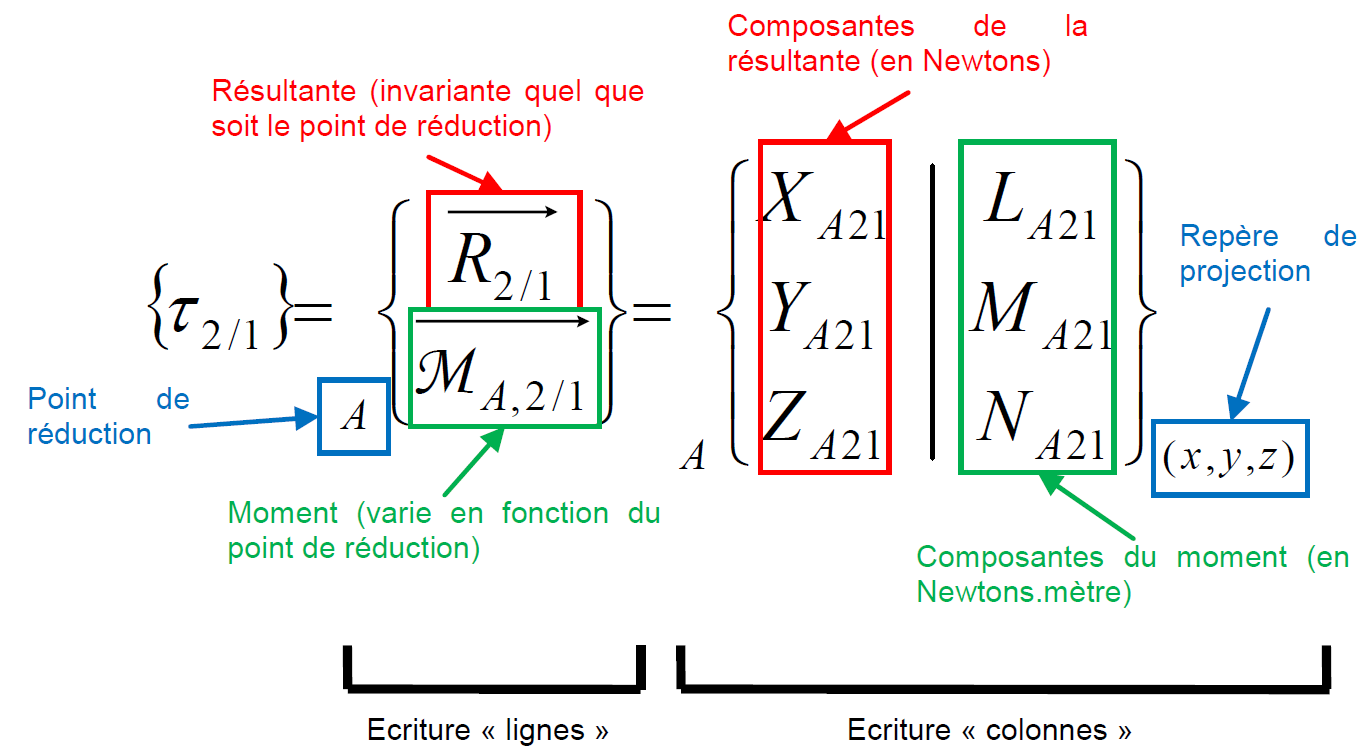
\includegraphics[width=0.8\textwidth]{DD23.png}
        \end{center}

\end{document}